\documentclass{article}

% if you need to pass options to natbib, use, e.g.:
% \PassOptionsToPackage{numbers, compress}{natbib}
% before loading nips_2016
%
% to avoid loading the natbib package, add option nonatbib:
% \usepackage[nonatbib]{nips_2016}

%\usepackage[final]{nips_2016}

% to compile a camera-ready version, add the [final] option, e.g.:
\usepackage[final]{nips_2016}

\usepackage[utf8]{inputenc} % allow utf-8 input
\usepackage[T1]{fontenc}    % use 8-bit T1 fonts
\usepackage{hyperref}       % hyperlinks
\usepackage{url}            % simple URL typesetting
\usepackage{booktabs}       % professional-quality tables
\usepackage{amsfonts}       % blackboard math symbols
\usepackage{nicefrac}       % compact symbols for 1/2, etc.
\usepackage{microtype}      % microtypography
\usepackage{amsmath}
\usepackage{amssymb}
\usepackage{graphicx}
\usepackage{bbm}

\title{Deep Q-Learning with Recurrent Neural Networks}

% The \author macro works with any number of authors. There are two
% commands used to separate the names and addresses of multiple
% authors: \And and \AND.
%
% Using \And between authors leaves it to LaTeX to determine where to
% break the lines. Using \AND forces a line break at that point. So,
% if LaTeX puts 3 of 4 authors names on the first line, and the last
% on the second line, try using \AND instead of \And before the third
% author name.

\author{
  Clare Chen \\
  \texttt{cchen9@stanford.edu} \\
  \And
  Vincent Ying \\
  \texttt{vincenthying@stanford.edu} \\
  \And
  Dillon Laird \\
  \texttt{dalaird@cs.stanford.edu} \\
}

% Remove NIPS footer
\pagestyle{empty}

\begin{document}
% \nipsfinalcopy is no longer used

\maketitle

\begin{abstract}
  Deep reinforcement learning models have proven to be successful at learning
  control policies image inputs. They have, however, struggled with learning
  policies that require longer term information. Recurrent neural network
  architectures have been used in tasks dealing with longer term dependencies
  between data points. We investigate these architectures to overcome the
  difficulties arising from learning policies with long term dependencies.
\end{abstract}


\section{Introduction}
    Recent advances in reinforcement Learning have led to human-level or greater
    performance on a wide variety of games (e.g. Atari 2600 Games). However,
    training these networks can take a long time, and the techniques presented in
    the state of the art [0] perform poorly on several games that require long
    term planning. \\
    \\
    Deep Q-networks are limited in that they learn a mapping from a single
    previous state which constist of a small number of game screens. In practice,
    DQN is trained using an input consisting of the last four game screens. Thus,
    DQN performs poorly at games that require the agent to remember information
    more than four screens ago. This is evident from the types of games DQN performs
    poorly at, near or below human-level [0], in Figure 1. \\
    \\
    We explore the concept of a deep recurrent Q-network (DRQN), a combination of
    a recurrent neural network (RNN) [6] and a deep Q-network (DQN) similar to [5]
    \footnote{code at \url{https://github.com/dillonalaird/deep-rl-tensorflow}}.
    The idea being that the RNN will be able to retain information from states
    further back in time and incorporate that into predicting better Q values
    and thus performing better on games that require long term planning. \\

    \begin{figure}[h]
        \centering
        \begin{minipage}{0.8\textwidth}
            \centering
            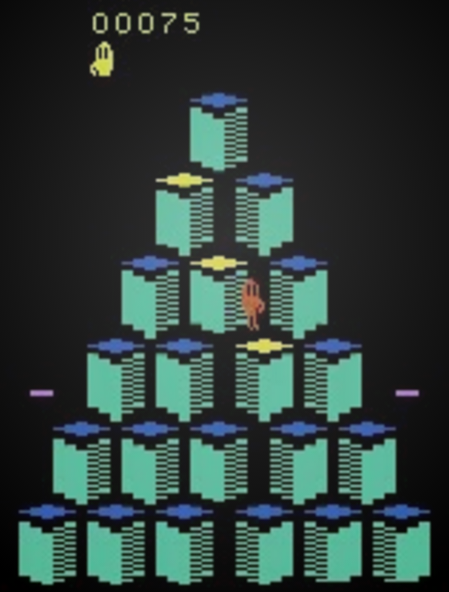
\includegraphics[scale=0.15]{Qbert}
            \centering
            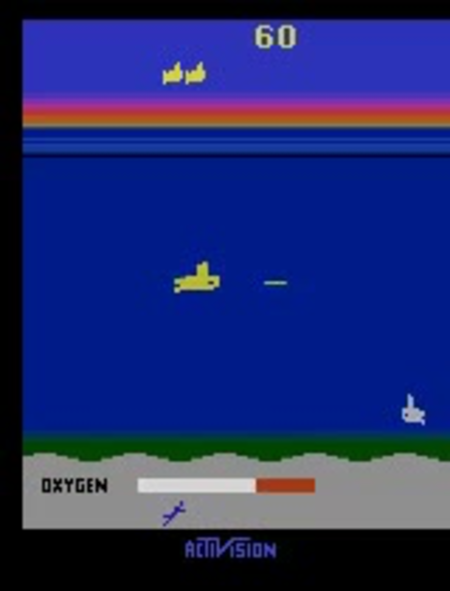
\includegraphics[scale=0.15]{Seaquest}
            \centering
            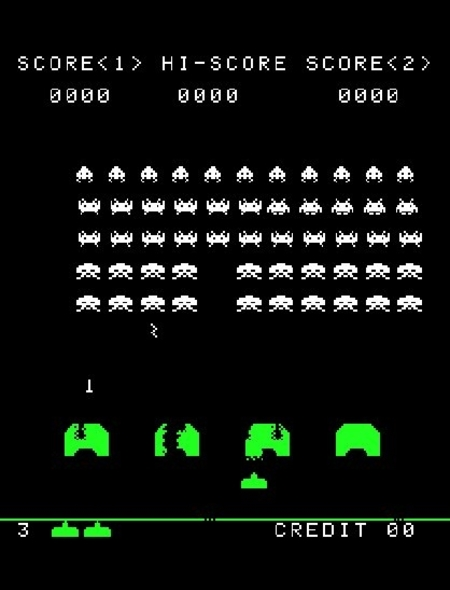
\includegraphics[scale=0.15]{SpaceInvaders}
            \centering
            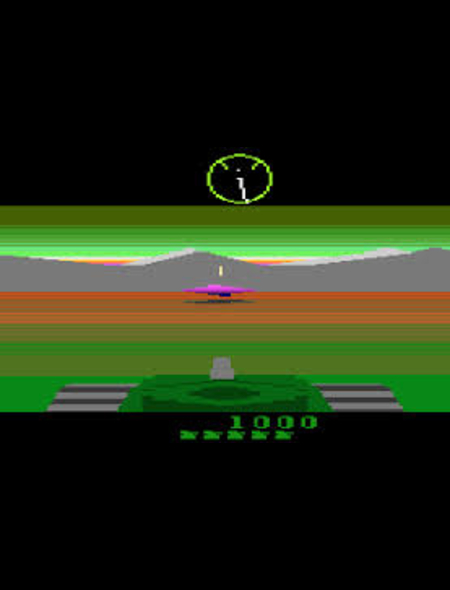
\includegraphics[scale=0.15]{BattleZone}
        \end{minipage}
        \caption{Q*bert, Seaquest, SpaceInvaders, and BattleZone}
    \end{figure}


    In addition to vanilla RNN architectures we also examine augmented RNN
    architectures such as attention RNNs. Recent achievments of attention RNNs in
    translation tasks [2, 3] have shown promise. The advantage of using attention
    is that it enables DRQN to focus on particular previous states it deems
    important for predicting the action in the current state. We investigate
    augmenting DRQN with attention and evaluate its usefulness.

\section{Relatd Work}

Reinforcement learning covers a variety of areas from playing backgommon [7] to
flying RC helicopters [8]. Traditionally reinforcement learning relied upon
iterative algorithms to train agents on smaller state spaces. Later, algorithms
such as Q-learning were used with non-linear function aproximators to train agents
on larger state spaces. These algorithms, however, were more difficult to train
and would diverge [9].

Recent advances in reinforcement learning have made it possible to use deep
neural networks as non-linear function approximators and train them without
running into stability issues. These types of models are known as Q-networks and
have been shown to be very successful at playing games such as Atari games where
the input is nothing more than the pixels on the screen [0, 1].

We examine extending this framework to include RNNs. RNNs have been used before
in Q-Learning [5] but on partially observable Markov decision processes created
by flickering the game screen. Our goal is to improve the average score the agent
receives.

\section{Deep Q-Learning}

We examine agents playing Atari games. In our environment the agents interact with
an Atari emulator. At time $t$ they recieve an observation $x_t \in \mathbb{R}^D$
which is a vector of pixels from the current game screen. The agent then takes an
action, $a_t \in \mathcal{A} = \{1, \dots, K\}$ and receives a reward $r_t$ which
is the change in the game score. \\
\\
The objective of the agent is to take actions that maximize the future discounted
rewards. We can calculate the future rewards with $R_t = \sum_{t' = 1}^T \gamma^{t'-1}r_{t'}$
where $T$ is the end of the game and $\gamma$ is our discount factor. One way
to achieve this objective is by taking the action corresponding to the maximum
action-value function:
$$Q^*(s,a) = \max_{\pi}\mathbb{E}[r_t + \gamma r_{t+1} + \gamma^2 r_{t+2} + \dots
|s_t = s, a_t = a, \pi]$$
which is the expected value of the future discounted rewards under the policy
$\pi = P(a|s)$, or the probability of taking an action given the agent is in a
certain state. Unfortunately this method can be very difficult to calculate it
so we approximate it with another function $Q(s,a;\theta) \approx Q^*(s,a)$. We
examine several different types of deep neural network architectures for our
function approximator which are called Q-networks. \\
\\
Training this function can be unstable and will sometimes diverge. The following
following loss function is used to help reduce some of these issues [0]:
\begin{equation}
    L_i(\theta_i) = \mathbb{E}_{(s,a,r,s') \sim U(D)}\Big[\Big(
    r + \gamma \max_{a'}Q(s',a';\theta_i^-) - Q(s,a;\theta_i)\Big)^2\Big]
\end{equation}

Where experiences are defined as $e_t = (s_t, a_t, r_t, s_{t+1})$ and the buffer
in which experiences are stored is $D_t = \{e_1, \dots, e_t\}$. In the SGD update
we sample minibatches of experience tuples $(s, a, r, s') \sim U(D)$ which are
drawn uniformly at random from the memory buffer. This is called experience replay
and is designed to mitigate instability in the training process. In the loss
function above, $\theta_i^-$ are the network parameters used to compute the target
network at iteration $i$. We only update these target network parameters with
the $Q$-network parameters $\theta_i$ every $C$ steps; note that we are keeping a
$Q$-network and a target network.

\section{Deep Recurrent Q-Learning}

We examine several architectures for the DRQN. The idea behind using a RNN on top
of a DQN is to retain information for longer periods of time. This should help the
agent accomplish tasks that may require the agent to remember a particular event
that happened several dozens screen backs. We also examine using an attention
mechanism in the RNN. Attention allows the RNN to focus on particular states it
has seen in the past. One can think of it as assigning importance to the states
iterated over by the RNN. We investigate $2$ forms of attention; A linear attention
that uses a learned vector to assign importances over the previous states and a
global attention that assigns importances to previous states based on the current
state. \\
\\
The first architecture is a very basic extension of DQN. The architecture of DRQN
augments DQN's fully connected layer with a LSTM. We accomplish this by looking at
the last $L$ states, $\{s_{t-(L-1)}, \dots, s_{t}\}$ and feed these into a
convolutional neural network (CNN) to get intermediate outputs
$\text{CNN}(s_{t-i}) = x_{t-i}$. These are then fed into a RNN (we use an LSTM for
this but it can be any RNN), $\text{RNN}(x_{t-i}, h_{t-i-1}) = h_{t-i}$, and the
final output $h_t$ is used to predict the $Q$ value which is now a function of
$Q(\{s_{t-(L-1)}, \dots, s_t\}, a_t)$.

\begin{figure}[h]
    \centering
    \includegraphics[scale=0.3]{DRQN_attn}
    \caption{Architecture of the Attention DRQN}
\end{figure}

The second architecture we used was a version of an attention RNN we are calling 
linear attention. For the linear attention RNN we take the $L$ hidden states
outputted by the RNN, $\{h_{t-(L-1)}, \dots, h_{t}\}$ and calculate an inner
product with $v_a$, $\{v_a^Th_{t-(L-1)}, \dots, v_a^Th_{t}\}$. This allows the
model to focus more on nearby hidden states or further away states depending on
what values of $v_a$ are learned. We then take a softmax over these values,
$a_{t-i} = \text{softmax}(v_a^Th_{t-i})$. We use this softmax to take a weighted
sum over the hidden states to get a context vector,
$c_t = \sum_{i=0}^{L-1}a_{t-i}h_{t-i}$. This context vector is then used to predict
the $Q$ value. \\
\\
The third architecture we used is global attention, similar to the global attention
used in [3]. A diagram of this type of attention can be seen in Figure 2. We treat
the current state, $s_t$ as the "decoder" input and the previous $L - 2$ states as
the "encoder" inputs. We compute the following scores,
$\{{h_{t-(L-1)}}^Th_t, \dots, {h_{t-1}}^Th_t\}$. We then take a softmax over these
values, $a_{t-i} = \text{softmax}({h_{t-i}}^Th_t)$. The context vector is computed
as a weighted sum over the previous hidden states, $c_t = \sum_{i=1}^{L-1}a_{t-i}h_{t-i}$.
Finally the context vector is used to compute $\tilde{h} = \tanh(W_a[h_t;c_t] + b_a)$
which is then used to predict the $Q$ value. This type of attention allows the model
to focus on previous states depending on the current state $h_t$ as opposed to a
fixed vector such as $v_a$. \\
\\
Learning sequences of observations creates some difficulty when sampling
experiences and using the loss function defined in (1). We propose a simple
solution where we sample $e_t \sim U(D)$ and then take the previous $L$ states,
$\{s_{t-(L+1)}, \dots, s_t\}$ and zero out states from previous games. For example
if $s_{t-i}$ was the end of the previous game then we would have states
$\{\mathbf{0}, \dots, \mathbf{0}, s_{t-(i+1)}, \dots, s_t\}$ and similarly for the
next state $\{\mathbf{0}, \dots, \mathbf{0},s_{t-(i+2)}, \dots, s_{t+1}\}$.

\section{Experiments}

For our experiments we mainly focused on the game Q*bert. We chose Q*bert because
it was a challenging game for DQN which achieved scores only slightly above
human-level [0] but it was not so challenging that DQN could not make any progress,
such as Montezuma's Revenge [0]. \\
\\
For input the DRQN takes a specified number of screens per state. The screen images
are grayscaled and resized to $80 \times 80$. The first hidden layer convolves $16$,
$19 \times 19$ filters with stride $8$ across the input image and applies a rectified
linear unit.  The second hidden layer convolves $32$, $8 \times 8$ filters with
stride $4$, again followed by a rectified linear unit.  Convolutional outputs are
fed to an LSTM with $256$ hidden units per layer.  Finally, a fully connected
linear layer outputs a Q-value for each possible action. All of the hyperparameters
used are listed in Apendix A. These are similar to the hyperparameters used in [0]. \\

\begin{figure}[h]
    \centering
    \begin{minipage}{1.0\textwidth}
        \centering
        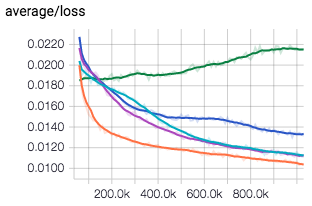
\includegraphics[scale=0.2]{avg_loss}
        \centering
        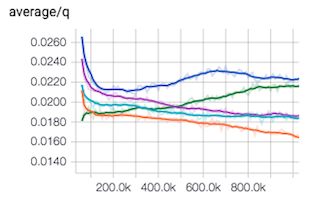
\includegraphics[scale=0.2]{avg_q}
        \centering
        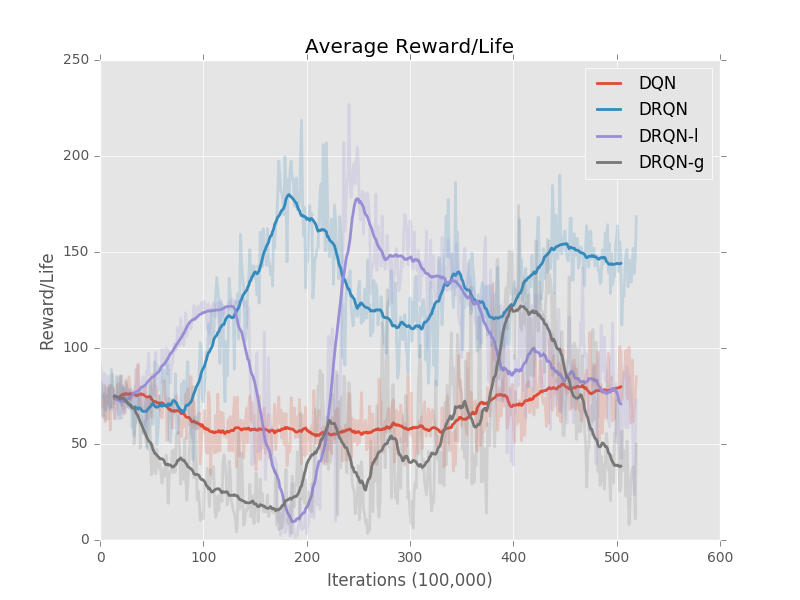
\includegraphics[scale=0.2]{avg_reward}
    \end{minipage}
    \caption{Graphs for Q*bert Over 5 Million Iterations}
\end{figure}

\begin{figure}[h]
    \centering
    \begin{minipage}{1.0\textwidth}
        \centering
        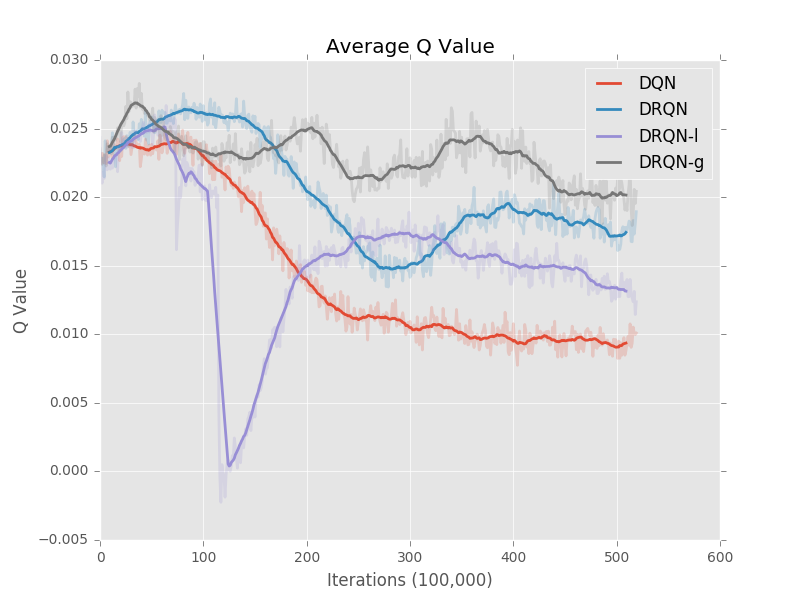
\includegraphics[scale=0.2]{Seaquest1}
        \centering
        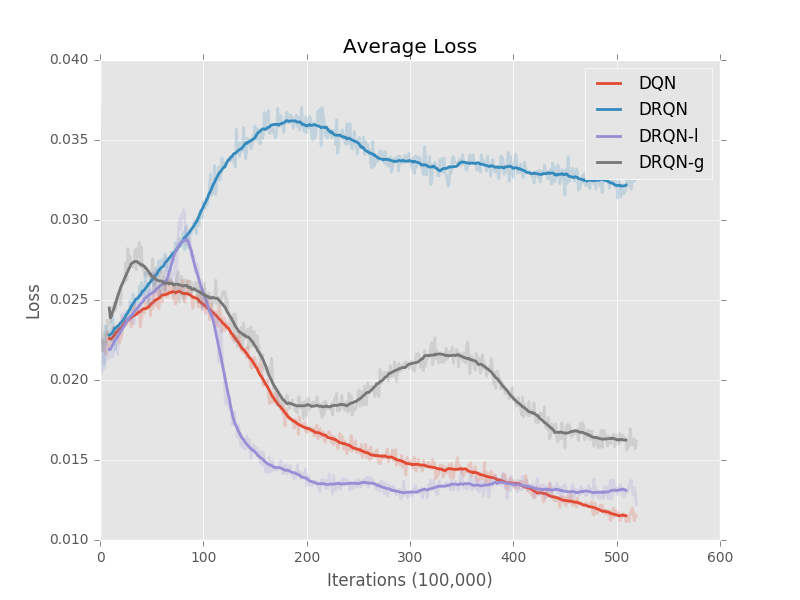
\includegraphics[scale=0.2]{Seaquest2}
        \centering
        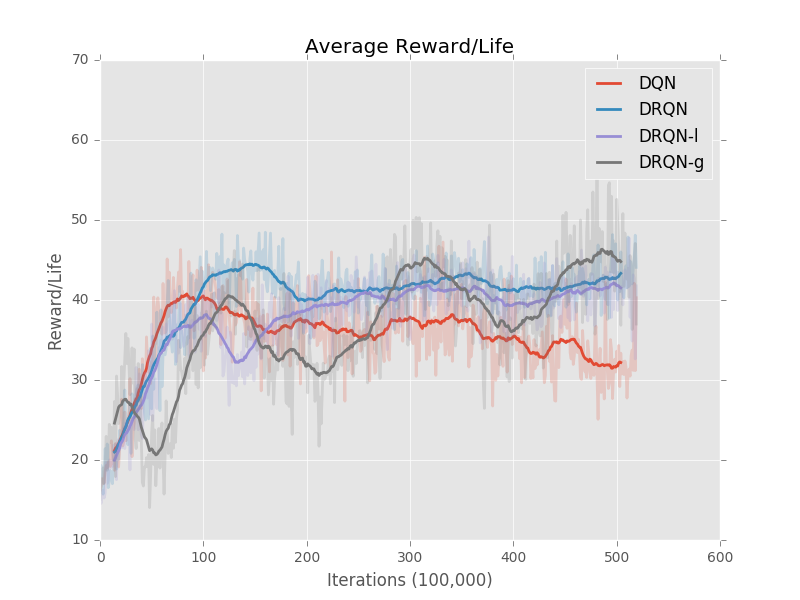
\includegraphics[scale=0.2]{Seaquest3}
    \end{minipage}
    \caption{Graphs for Seaquest Over 5 Million Iterations}
\end{figure}

For Figure 3 we trained $4$ different models for about $5$ million iterations on
Q*bert which took about $6$ days to complete. All the models use the same
convolutional neural network described above for processing the images. DQN uses
$4$ game screens per state. \\
\\
The DRQN models in Figure 3 used $L=16$ and $2$ screens per state which allows it
to see the last $32$ frames. We wanted to give the model let the model look over
enough previous states to more informed decision but not so many that RNN suffers
from vanishing or exploding gradients and training time issues which is why we
chose $L=16$. We found $2$ screens per states to allow the model to run efficiently
without suffering in scores. DRQN is a basic recurrent model with no attention
mechanism. DRQN-l is the recurrent model with linear attention and DRQN-g is the
recurrent model with global attention. \\
\\
As you can see from Figure 3 the graphs for the DRQN models are very noisy. The
regular DRQN performed the best in terms of average points per life but also had
the most difficult time reducing the loss. DRQN-l had the noisiest graphs. It
peformed close to the highest and lowest value at some point on every statistic.
DRQN-g's performance was dissapointing. It had the easiest time minimizing the loss
but struggled to gain momentum on average reward per life. \\

\begin{figure}[h]
    \begin{center}
        \begin{tabular}{| c | c | c | c | c |}
            \hline
            & \textbf{Q*bert} & \textbf{Seaquest}  \\ \hline
            \textbf{DQN} & 700 & 360  \\ \hline 
            \textbf{DRQN} & \textbf{850} & 360 \\ \hline
            \textbf{DRQN-l} & 700 & \textbf{620} \\ \hline
            \textbf{DRQN-g} & 550 & 380 \\ \hline
        \end{tabular}
    \end{center}
    \caption{Best Scores for Trained Atari Games}
\end{figure}

In Figure 4 we can see the best scores received from each of the algorithms playing
$100$ games of Q*bert. This table reflects where the algorithms ended up in the
average rewards per life graph in Figure 3 with DRQN peforming the best followed
by DQN, DRQN-l and finally DRQN-g. Unfortunately we were not able to reproduce the
score achieved by [1] on Q*bert. \\
\\
From these figures it is evident that while adding a recurrent layer helped the
agent, adding an attention mechanism only hidnered the agent. We hypothesize
several reasons that explain the poorer results. For one, the network that must
be trained is bigger, there are more parameters to tune and it is apparent from
the graphs that the attention DRQN did not converge. It is possible that training
it longer would lead to better results. Another reason is that attention is not
necessary for playing Q*bert since the agent receives the full game state on each
screen it does not need to focus on game screens too far back.

\section*{Conclusion}

We investigate using an RNN on top of a DQN (DRQN) and test several different types
of attention to augment the RNN. We show that a basic DRQN is capable of achieving
better scores than a DQN on a game that is difficult for DQN to play. We also
show that adding attention can hinder the performance on certain games as well. \\
\\
Going forward we would have liked to train the algorithms for even longer to see
if attention eventually does perform better. It is apparent that the graphs have
not converged and are still very noisy. We also think running the agent on games
where the game state is not fully revealed in the screen would better utilize
attention to achieve higher scores. Think of a game where in one screen you see
a person and in the next screen they run behind a wall. The agent should attend
to the screen where the person was last visible to gain information about where
they might be in the current frame.

\section*{Acknowledgements}

We would like to thank carpedm20 for using his DQN repository as a base for
running our experiments. It saved us a lot of time and allowed us to focus on the
core part of our experiment which was testing DRQN.

\section*{Appendix A:}

\begin{tabular}{ |l|l|l| }
  \hline
  \multicolumn{3}{|c|}{List of Hyperparameters} \\
  \hline
  minibatch size & 32 & number of experiences for SGD update\\
  replay memory buffer size & 1000000 & number of experiences in memory buffer\\
  agent history length & 4-32 & number of most recent frames experienced input to the Q network\\
  target network update frequency & 10000 & number of parameter updates after which the target network updates\\
  discount factor & 0.99 & Discount factor $\gamma$ used in the Q-learning update\\
  action repeat & 4 & Repeat each action selected by the agent this many times\\
  update frequency & 4 & number of actions by agent between successive SGD updates. \\
  initial exploration & 1 & Initial value of $\epsilon$ in $\epsilon$-greedy exploration \\
  final exploration & 0.01 & Final value of $\epsilon$ in $\epsilon$-greedy exploration\\
  final exploration frame & 100000 & The number of frames over which the initial value of $\epsilon$ reaches final value\\
  no-op max & 30 & Maximum "do nothing" actions by agent at the start of episode.\\
  learning rate of training & 0.00025 & learning rate used by RMSProp\\
  decay of RMSProp optimizer & 0.99 & decay rate used by RMSProp\\
  $\beta$ of RMSProp optimizer & 0.01 & $\beta$ rate of RMSProp\\
  \hline
\end{tabular}

\section*{References}
\small
% TODO: need to figure out how to cite this stuff properly..
[0] Volodymyr Mnih, Koray Kavukcuoglu, David Silver, Andrei A. Rusu, Joel Veness, Marc G. Bellemare, Alex Graves, Martin Riedmiller, Andreas K. Fidjeland, Georg Ostrovski, Stig Petersen, Charles Beattie, Amir Sadik, Ioannis Antonoglou, Helen King, Dharshan Kumaran, Daan Wierstra, Shane Legg, and Demis Hassabis. Human-level Control through Deep Reinforcement Learning. {\it Nature}, 518(7540):529-522, 2015.

[1] Volodymyr Mnih, Koray Kavukcuoglu, David Silver, Alex Graves, Ioannis Antonoglou, Daan Wierstra and Martin Riedmiller. Playing Atari with Deep Reinforcement Learning. {\it arXiv preprint arXiv:1312.5602}, 2013.

[2] Dzmitry Bahdanau, Kyunghyun Cho and Yoshua Bengio. Neural Machine Translation by Jointly Learning to Align and Translate. {\it arXiv preprint arXiv:1409.0473}, 2014.

[3] Minh-Thang Luong, Hieu Pham and Chisopher D. Manning. Effective Approaches to Attention-based Neural Machine Translation. {\it arXiv preprint arXiv:1508.04025}, 2015.

[4] Ivan Sorokin, Alexey Seleznev, Mikhail Pavlov, Aleksandr Fedorov and Anastasiia Ignateva. Deep Attention Recurrent Q-Network. {\it arXiv preprint arXiv:1512.01693}, 2015.

[5] Matthew Hausknecht and Peter Stone. Deep Recurrent Q-Learning for Partially Observable MDPs. {\it arXiv preprint arXiv:1507.06527}, 2015.

[6] Sepp Hochreiter and Jurgen Schmidhuber. Long Short-Term Memory. {\it Neural Computation}, 9(8):1735-1780, 1997.

[7] Gerald Tesauro. Temporal difference learning and td-gammon. {\it Communications of the ACM}, 38(3):58-68, 1995.

[8] Andrew Y. Ng, H. Jin Kim, Michael I. Jordan and Shankar Sastry. Autonomous Helicopter Flight via Reinforcement Learning. {\it Advances in Neural Information Processing Systems 16}, 2003.

[9] John N. Tsitsiklis and Benjamin Van Roy. An analysis of temporal-difference learning with function approximation. {\it Automatic Control, IEEE Transactions on}, 42(5):647-690, 1997.


\end{document}
